\chapter{The Zeta Function of Riemann (Contd).}\label{chap12}

\setcounter{section}{5}
\section[Some estimates for $\zeta(s)$]{Some estimates for {\boldmath$\zeta(s)$} \cite[p.27]{key11}}\label{chap12:sec6}\pageoriginale 

In any fixed half-plane $\sigma\geq 1 + \epsilon >1$, we know that
$\zeta(s)$ is bounded, since 
$$
|\zeta (s)| \leq \zeta(\sigma) \leq \zeta (1+ \epsilon).
$$
We shall now use the formulae of \S\ 5 to estimate $|\zeta(s)|$ for
large $t$, where $s = \sigma + it$.

\begin{theorem*}
\begin{align*}
& |\zeta(s)| < A \log t, \quad \sigma \geq 1, \quad t \geq 2. \\
& |\zeta(s)| < A (\delta) t^{1-\delta}, \quad \sigma \geq \delta,
  \quad t \geq 1, \text{ if~~ } 0 < \delta < 1.
\end{align*}
\end{theorem*}

\begin{proof}
From (\ref{chap11:subsec5.1}) we get
$$
\zeta(s) = \frac{s}{s-1} - s\int\limits^\infty_1 \frac{x-[x]}{x^{s+1}}
dx, \quad \sigma >0
$$

Also from \S\ 5 of the \ref{chap11}th Lecture,
$$
\sum\limits_{n \leq X} \frac{1}{n^s} = s \int\limits^X_1
\frac{[x]}{x^{s+1}} dx + \frac{[X]}{X^s}, \text{ if } X \geq 1, s \neq 1
$$
If $\sigma > 0$, $t \geq 1$, $X \geq 1$, we get 
$$
\zeta(s) - \sum_{n \leq X} \frac{1}{n^s} = -s \int\limits^\infty_X
\frac{x-[x]}{x^{s+1}} dx + \frac{1}{(s-1)X^{s-1}} + \frac{X-[X]}{X^s}
$$
Hence
\begin{align*}
|\zeta(s)| &<\sum\limits_{n \leq X} \frac{1}{n^{\sigma}} 
+ \frac{1}{t X^{\sigma -1}} + \frac{1}{X^\sigma} +|s|
\int\limits^\infty_{X} \frac{dx}{x^{\sigma +1}}\\
&< \sum\limits_{n \leq X} \frac{1}{n^\sigma} + \frac{1}{tx^{\sigma-1}}
+ \frac{1}{X^{\sigma}} + \left(1+ \frac{t}{\sigma} \right)
\frac{1}{X^\sigma}, \text{ since } |s| < \sigma +t.
\end{align*}\pageoriginale
If $\sigma \geq 1$,
\begin{align*}
|\zeta(s)| & < \sum\limits_{n \leq X} \frac{1}{n}+ \frac{1}{t} +
\frac{1}{X} + \frac{1+t}{X}\\
& \leq (\log X +1) + 3 + \frac{t}{X}, \text{ since } t \geq 1,\quad X
\geq 1.
\end{align*}
Taking $X=t$, we get the first result.

If $\sigma \geq \eta$, where $0< \eta <1$,
\begin{align*}
|\zeta(s)| & < \sum\limits_{n \leq X} \frac{1}{n^\eta} +
\frac{1}{tX^{\eta-1}} + \left(2+\frac{1}{\eta} \right)
\frac{1}{x^\eta}\\
& < \int\limits^{[X]}_0 \frac{dx}{x^\eta} + \frac{X^{1-\eta}}{t} +
\frac{3t}{\eta X^\eta}\\
& \leq \frac{X^{1-\eta}}{1-\eta} + X^{1-\eta} + \frac{3t}{\eta X^\eta}
\end{align*}

Taking $X =t$, we deduce
$$
|\zeta(s)| < t^{1-\eta} \left(\frac{1}{1-\eta} + 1 + \frac{3}{\eta}
\right), \quad \sigma \geq \eta, \quad t \geq 1.
$$
\end{proof}

\section[Functional Equation (Third Method)]{Functional Equation (Third Method) \cite[p.21]{key16}}\label{chap12:sec7}
The third method is based on the `theta-relation'
$$
\vartheta(x) = \frac{1}{\sqrt{x}} \vartheta\left(\frac{1}{x} \right),
$$
where 
$$
\vartheta (x) = \sum\limits^\infty_{n = - \infty} e^{-\pi n^2x}, \re x > 0
$$
This\pageoriginale relation can be proved directly, or obtained as a
special case of `\textit{Poisson's formula}'. We shall here give a
proof of that formula \cite[p.37]{key2}

Let $f(x)$ be continuous in $(-\infty, \infty)$. Let
$$
\phi(\alpha) = \int\limits^\infty_{-\infty} f(x) e^{2 \pi i \alpha x}
dx \equiv \lim\limits_{T \to \infty} \int\limits^T_{-T} f(x) e^{2\pi i
\alpha x} dx,
$$
if the integral exists. Then, for \textit{$\alpha$ and $p$, positive
  integers}, we have
\begin{equation}
\int\limits^{p+\frac{1}{2}}_{-p-\frac{1}{2}} f(x) e^{2\pi i \alpha
  x}dx = \int\limits^{\frac{1}{2}}_{-\frac{1}{2}}
\left\{\sum\limits^p_{-p} f (x+k) \right\} e^{2\pi i \alpha x}dx.\label{c12:eq7.1}
\end{equation}
If we assume that 
\begin{equation*}
\lim\limits_{p\to\infty} \sum\limits^p_{-p} f(x+k) = g(x)
\end{equation*}
\textit{uniformly} in $-\frac{1}{2} \leq x \leq \frac{1}{2}$, then
$g(x)$ is continuous, and on letting $p\to \infty$ in \eqref{c12:eq7.1}, we get
$$
\phi (\alpha) = \int\limits^{\frac{1}{2}}_{-\frac{1}{2}} g(x) e^{2\pi
  i \alpha x} dx.
$$
Thus $\phi(\alpha)$ is the Fourier coefficient of the continuous
periodic function $g(x)$. Hence, by Fejer's theorem,
$$
g(o) = \sum\limits_{(C,1)} \phi (\alpha)
$$
If we assume, however, that $\sum\limits^\infty_{-\infty} \phi (\alpha)
< \infty$, then $\sum\limits_{(C,1)} \phi (\alpha) =
\sum\limits^\infty_{-\infty} \phi (\alpha)$ 
Hence
$$
\lim\limits_{p\to \infty} \sum\limits^p_{-p} f(k) =
\lim\limits_{p\to\infty} \sum\limits^p_{-p} \phi (\alpha)
$$
or\pageoriginale
\begin{equation}
\sum\limits^\infty_{-\infty} f(k) = \sum\limits^\infty_{-\infty} \phi
(\alpha)\label{c12:eq7.2}
\end{equation}
This is Poisson's formula. We may summarize our result as
follows. \textit{Poisson's Formula}. If
\begin{itemize}
\item[{\rm(i)}] $f(x)$ is continuous in $(-\infty, \infty)$,

\item[{\rm(ii)}] $\sum\limits^\infty_{-\infty} f(x+k)$ converges
  uniformly in $-\frac{1}{2} \leq x < \frac{1}{2}$ and 

\item[{\rm(iii)}] $\sum\limits^\infty_{-\infty} \phi (\alpha)$ converges,
\end{itemize}
then \  
$
\sum\limits^\infty_{-\infty} f(k) = \sum\limits^\infty_{-\infty} \phi
(\alpha) 
$

\begin{remarks*}
This result can be improved by a relaxation of the hypotheses.
\end{remarks*}


\medskip
\noindent{\textbf{The Theta Relation.}}
If we take $f(x) =e^{-\pi x^2t}$, $t >0$, in the above discussion, we
obtain the required relation. However, we have to show that for this
function the conditions of Poisson's formula are satisfied. This is
easily done. $f(x)$ is obviously continuous in $(-\infty,
\infty)$. Secondly
$$
e^{-\pi(x+k)^2t} \leq e^{|k|t} \text{ for } |k| \geq k_0 (t)
$$

This proves the uniform convergence of 
$$
\sum\limits^\infty_{k=-\infty} e^{-\pi(x+k)^2t} , \quad t >0,\quad -
\frac{1}{2} \leq x < \frac{1}{2}
$$
Thirdly we show that, for $t>0$
$$
\phi(\alpha) \equiv \int\limits^\infty_{-\infty} e^{-y^2 \pi t + 2 \pi
\alpha yi} dy = \frac{1}{t^{1/2}} e^{-\pi \alpha^2/t}
$$
For\pageoriginale
$$
\phi (\alpha) = e^{-\frac{\pi \alpha^2}{t}}
\int\limits^\infty_{-\infty} e^{-\pi t} \left(y-\frac{\alpha}{t}i
\right)^2 \; dy, \text{ and }
$$
If $\alpha \gtrless 0$, we consider the contour integral
$$
\int\limits_C e^{-\pi t s^2} ds, \quad s = \sigma + i \tau
$$
taken over $C$ as indicated. Then on the vertical lines, we have
\begin{figure}[H]
\centering
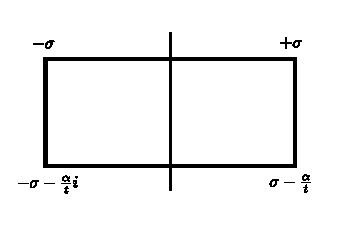
\includegraphics{figures/fig12.1.eps}
\end{figure}
$$
e^{-\pi t \re (\pm \sigma + \tau i)^2}  = e^{-\pi t (\sigma^2 -
  \tau^2) } \leq e^{-\pi t (\sigma^2 - \frac{\alpha^2}{t^2})} 
$$

Letting $\sigma \to \infty$, we thus see that the integrals along the
vertical lines vanish. Hence we have, for all real $\alpha$,
$$
\int\limits^\infty_{-\infty} e^{-\pi t \sigma^2} d\sigma =
\int\limits^\infty_{-\infty} e^{-\pi t (\sigma - \frac{\alpha}{t}i)^2}
d \sigma
$$
Thus
\begin{align*}
\phi (\alpha) & = e^{-\pi \alpha^2/t} \int\limits^\infty_{-\infty}
e^{-\pi t \sigma^2} d\sigma\\
& = e^{-\pi \alpha^2/t} \frac{1}{\sqrt{t}} \int\limits^\infty_{-\infty}
e^{-\pi u^2 } du\\
& = \frac{e^{-\pi \alpha^2 /t}}{\sqrt{t}} \frac{2}{\sqrt{\pi}}
\int\limits^\infty_0 e^{-\nu^2} dv = \frac{e^{-\pi \alpha^2/t}}{\sqrt{t}} \frac{1}{\pi} \int\limits^\infty_{0} e^{-z} z^{-\frac{1}{2}} dz\\
& = \frac{e^{-\pi\alpha^2/t}}{\sqrt{t}} \frac{1}{\sqrt{\pi}} \Gamma
\left(\frac{1}{2}\right) = \frac{e^{-\pi \alpha^2/t}}{\sqrt{t}}
\end{align*}

Hence\pageoriginale we have the desired relation:
\begin{equation}
\text{\fbox{$\sum\limits^\infty_{-\infty} e^{-\pi k^2 t} =
    \frac{1}{\sqrt{t}} \sum\limits^\infty_{-\infty} e^{-\pi k^2/t},$
    for $t>0$,}}\label{c12:eq7.3}
\end{equation}
or, writing
\begin{align}
\psi (t) &= \sum\limits^\infty_1 e^{-\pi k^2 t} , \text{ we get}\notag\\
2 \psi (t) + 1 &= \frac{1}{\sqrt{t}} \left\{2\psi \left(
\frac{1}{t}\right)+1 \right\} \label{c12:eq7.4}
\end{align}
Remark. (\ref{c12:eq7.3}) holds for $t$ complex, with $\re (t)>0$. 


\medskip
\noindent{\textbf{Functional Equation (Third method).}}

We have, for $\sigma >0$,
$$
\Gamma \left( \frac{s}{2}\right) = \int\limits^\infty_0 e^{-x}
x^{s/2-1} dx .
$$
If $\sigma >0$, $n>0$, we then have on writing $\pi n^2 x$ for $x$,
\begin{align*}
\Gamma \left(\frac{s}{2} \right) & = \int\limits^\infty_0 e^{-\pi n^2
  x} (\pi n^2 x)^{\frac{s}{2} -1} \pi n^2 dx\\
& = \pi^{s/2} n^s \int\limits^\infty_0 e^{-\pi n^2 dx } x^{s/2-1} dx\\
\text{or } \quad \frac{1}{n^s} & = \frac{\pi^{s/2}}{\Gamma(s/2)}
\int\limits^\infty_0 e^{-\pi n^2 x} x^{s/2 -1} \; dx.
\end{align*}

Now\pageoriginale \textit{if $\sigma >1$}, we have
\begin{align*}
\zeta(s) = \sum\limits^\infty_1 \frac{1}{n^s} & =
\frac{\pi^{s/2}}{\Gamma(s/2)}  \sum\limits^\infty_{n=1}
\int\limits^\infty_0 e^{-\pi n^2 x} x^{s/2-1} dx\\
& = \frac{\pi^{s/2}}{\Gamma(s/2)} \int\limits^\infty_0
\left(\sum\limits^\infty_1 e^{-\pi n^2 x} \right) x^{s/2 -1} dx
\end{align*}
the inversion being justified by absolute convergence. Hence, for
$\sigma >1$, we have 
$$
\zeta(s) = \frac{\pi^{s/2}}{\Gamma(s/2)} \int\limits^\infty_0 \psi(x)
x^{s/2 -1} dx.
$$
Using (\ref{c12:eq7.4}) we rewrite this as
\begin{align*}
&\pi^{-s/2} \Gamma (s/2) \zeta(s)  = \int\limits^1_0 x^{s/2-1} \psi(x)
  dx + \int\limits^\infty_1 \psi (x) x^{s/2-1} dx\\
&= \int\limits^1_0 x^{s/2 -1} \left\{\frac{1}{\sqrt{x}} \psi
  \left(\frac{1}{x} \right)  + \frac{1}{2\sqrt{x}} -
  \frac{1}{2}\right\}  dx + \int\limits^\infty_1 \psi (x) x^{s/2 -1}
  dx \\
& = \frac{1}{s-1} - \frac{1}{s} + \int\limits^1_0 x^{s/2 - 3/2} \psi
  \left(\frac{1}{x} \right) dx + \int\limits^\infty_1\\
& = \frac{1}{s(s-1)} + \int\limits^\infty_1 \left( x^{-s/2 -
    \frac{1}{2}} + x^{s/2-1}\right) \psi (x) dx , \tag{7.5}\label{c12:eq7.5}
\end{align*}
for $\sigma >1$.

Now\pageoriginale the integral on the right converges uniformly in $a
\leq s \leq b$, for if $x \geq 1$, we have
$$
\left|x^{-s/2-1/2} + x^{s/2-1} \right| \leq x ^{b/2-1} + x^{-a/2 -
  1/2} 
$$
while
$$
\psi (x) < \sum\limits^{\infty}_1 e^{-\pi n x} = \frac{1}{e^{\pi
    x}-1}, 
$$
and hence the integral on the right hand side of (\ref{c12:eq7.5}) is an entire
function. Hence (\ref{c12:eq7.5}) provides the analytic continuation to the left
of $\sigma =1$. It also yields the functional equation directly. We
have also deduced that
$$
\pi^{-s/2} \Gamma (s/2) \zeta(s) -\frac{1}{s(s-1)} 
$$
is an entire function; so is $\pi^{s/2} \{\Gamma(s/2)\}^{-1}$. Hence
$$
\zeta(s) - \frac{1}{s(s-1)} \cdot \frac{\pi^{s/2}}{\Gamma(s/2)} =
\zeta(s) - \frac{1}{s-1} \cdot \frac{\pi^{s/2}}{2 \Gamma(s/2 +1)}
$$
is an entire function. But $\dfrac{\pi^{1/2}}{2 \Gamma (1/2+1)}
=1$. Hence $\zeta(s) - \dfrac{1}{s-1}$ is an entire function.
